% четвертая часть

\section{Разработка пользовательского интерфейса мобильного приложения (UI/UX)}

Одна из важнейших задач в ходе создания мобильного приложения, преобразовывающего 2D снимки в объемные (3D) - разработка удобного и интуитивно-понятного пользовательского интерфейса. UI/UX (user Interface, user experience) составляющая, она же пользовательский интерфейс и пользовательский опыт, является более чем просто значимым элементом современного мобильного приложения. Удобство расположения элементов управления и приятное визуальное оформление напрямую влияют на настроение пользователя при использовании продукты. Именно некачественный UI/UX-дизайн отпугивает людей от использования многих приложений в пользу их более достойных альтернатив.

\subsection{Анализ интерфейсов смежных приложений}

Для использования в качестве референсов были подобраны приложения, принадлежащие широкому понятию «Приложения для работы с фото», так как узкоспециализированные решения не представляют интерфейса должного качества и удобства.

В список приложений для анализа попали такие приложения, как:  Prisma, Vinci, Snapster и Pixlr.

В первую очередь, целью сравнения являлся анализ особенностей пользовательского интерфейса этих приложений. Это обусловлено тем, что предполагаемая схема  взаимодействия пользователя с разрабатываемым приложением во много схожа с таковой в этих приложениях, за исключением некоторых их особенностей. Важные элементы для сравнения  - сценарий создания снимка с использованием фотокамеры смартфона и выбор снимка из галереи для дальнейшей отправки фотографии на обработку алгоритмом, преобразующим ее в 3D фотографию.

\subsubsection{Prisma}

Проанализировав пользовательский интерфейс первого приложения, Prisma (рисунок~\ref{fig:prisma}), можно заметить не очень удобное расположение элементов. Так, кнопка настроек, далеко не самая востребованная на фоне остальных, расположена в правом нижнем углу, куда доступ наиболее прост в условиях больших размеров современных смартфонов. В том время как кнопка смена камеры расположена в правом верхнем углу, куда доступ затруднительнее. Стоит отметить и факт смещения нижних иконок в углу экрана, что далеко не положительном образом сказывается на опыте использования приложения.

Также Prisma, в связи со своими социальными особенностями функционала, имеет навигационный бар в верхней части экрана, представленный фиксированными вкладками (fixed tabs), оформленным в соответствии с гайдлайнами material-дизайна (Material Design Guidelines), разработанными Google. В целом приложение лишь частично следует гайдлайнам от Google, что заметно на примере применения material-иконок и одновременно неверном использовании фаба (float action button).

Экран шейринга фотографии выполнен по примеру Instagram, с подобным размещением элементов и учетом особенностей Prisma.

\begin{figure}[H]
	\centering
	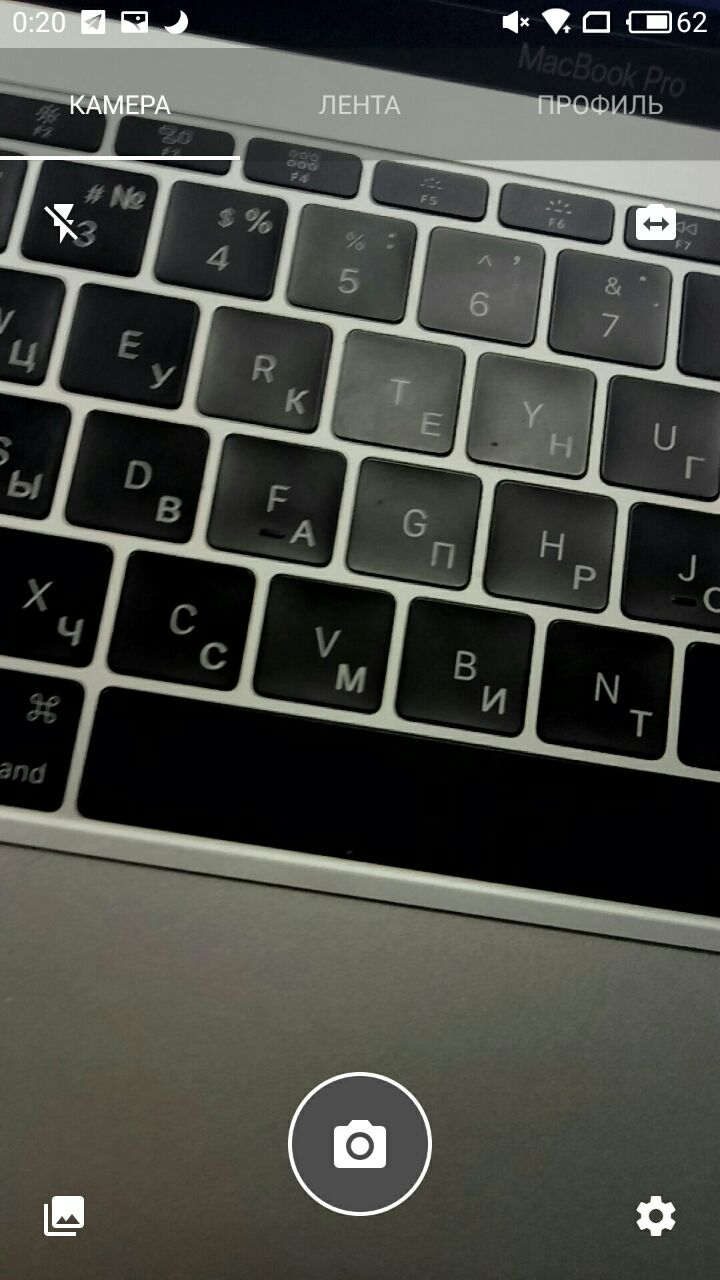
\includegraphics[width=0.45\linewidth]{pics/prisma1}
	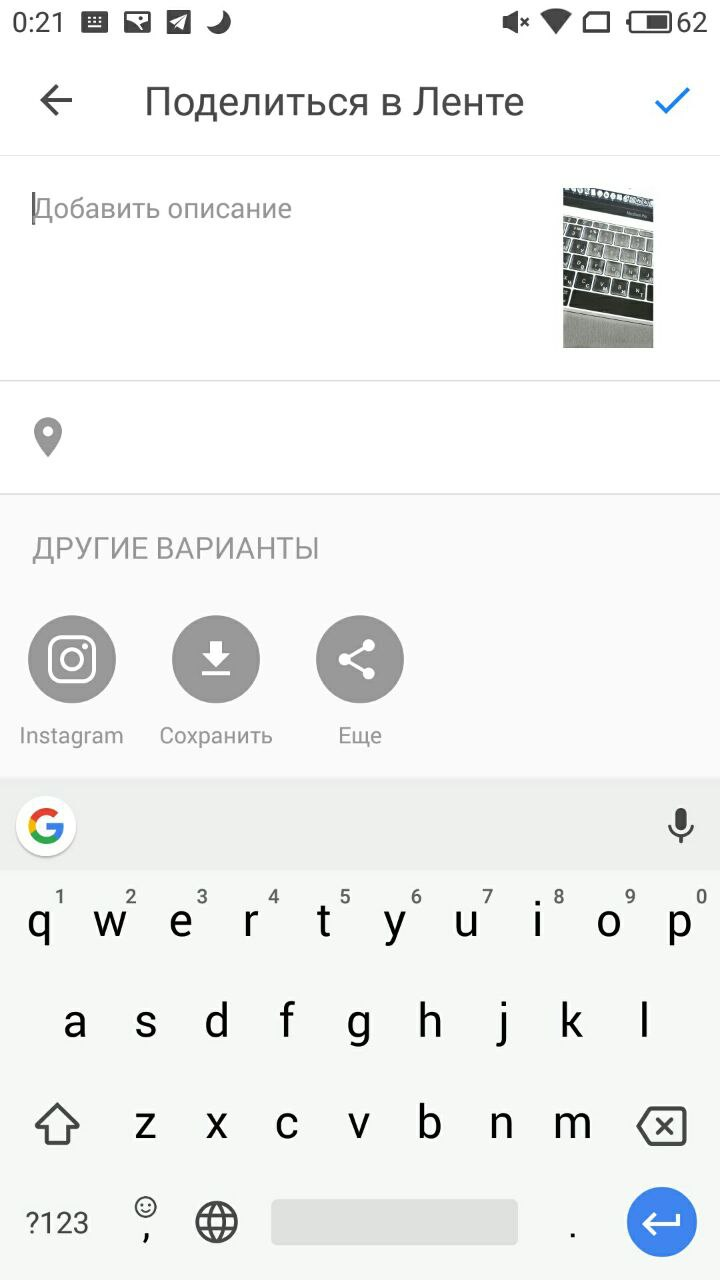
\includegraphics[width=0.45\linewidth]{pics/prisma2}
	\caption{Prisma}
	\label{fig:prisma}
\end{figure}

\subsubsection{Vinci}

Интерфейс Vinci (рисунок~\ref{fig:vinci}) выглядит более удачным, на фоне Prisma, и, забегая вперед, на фоне остальных выбранных приложений также, за исключением  Snapster. В нижней части удачно разместилась  выдвигающаяся панель с последними снимками, выше кнопка спуска затвора, включения вспышки и смены камеры. В верхнем углу разместилась иконка настроек. Такое разделение экрана обусловлено популярным соотношением сторон для снимков 4:3.

Плашка шейринга, появляющаяся в нижней части экрана, также весьма удобна для использования.

\begin{figure}[H]
	\centering
	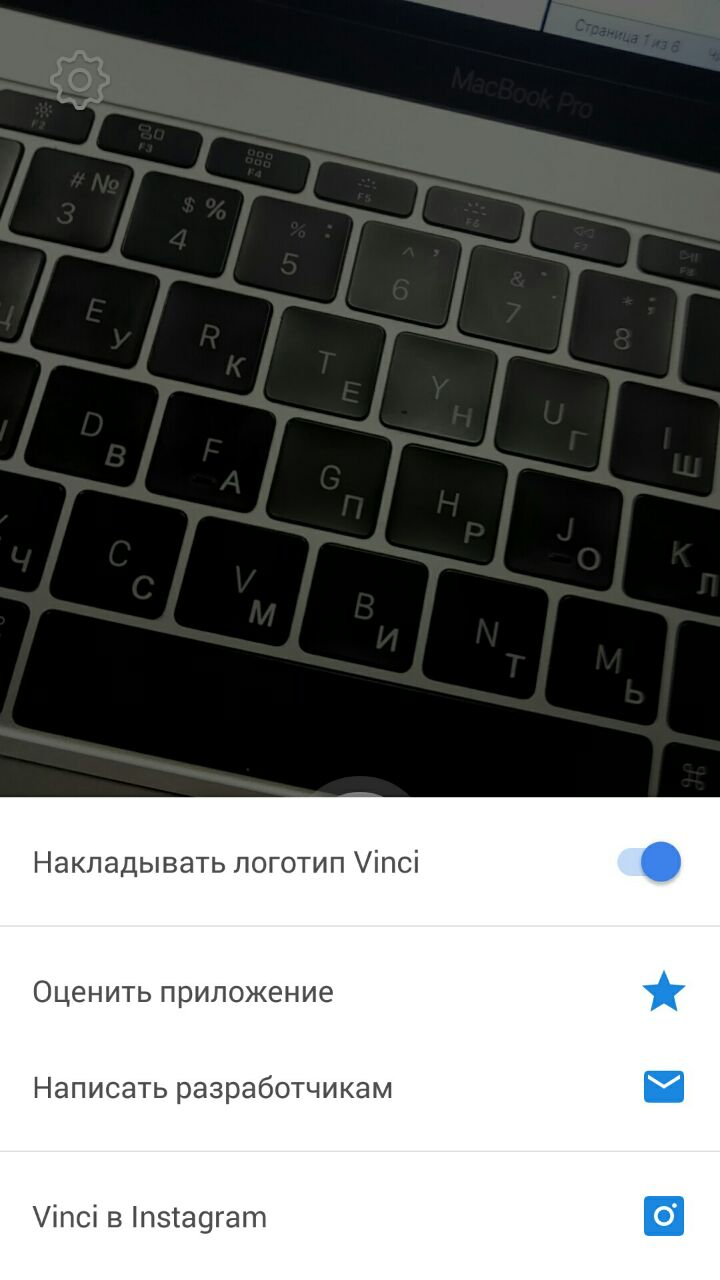
\includegraphics[width=0.3\linewidth]{pics/vinci1}
	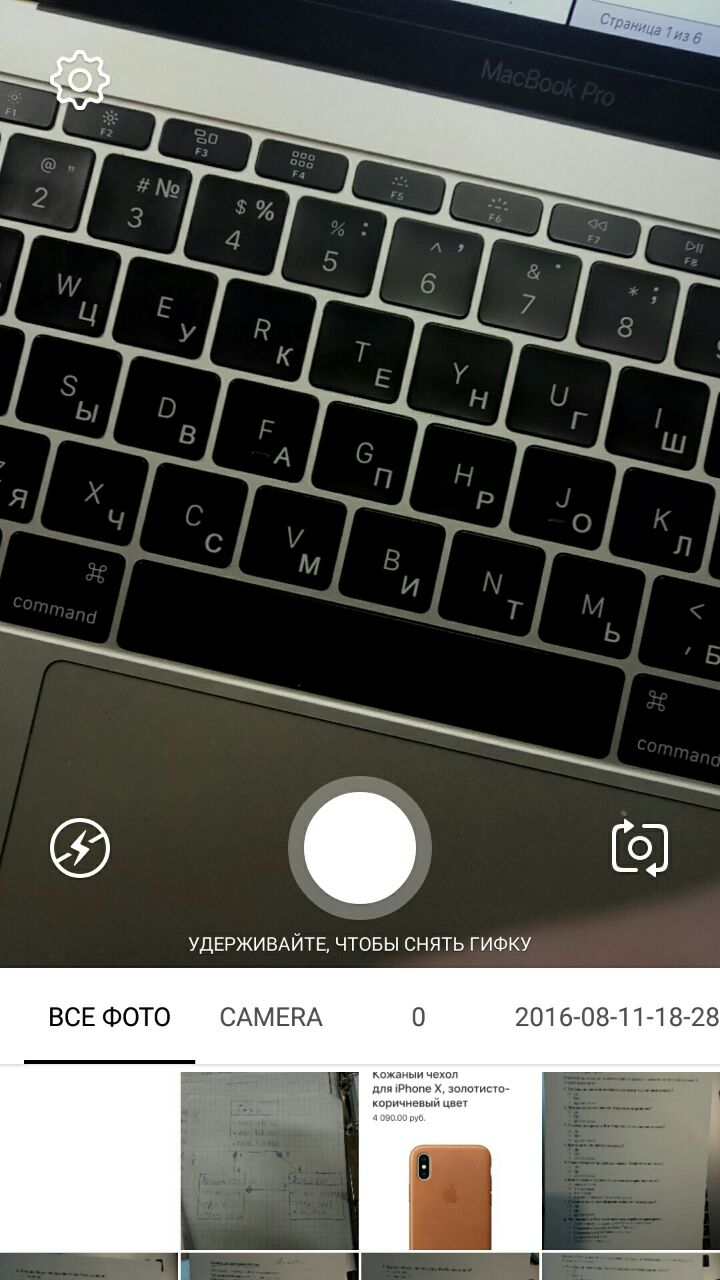
\includegraphics[width=0.3\linewidth]{pics/vinci2}
	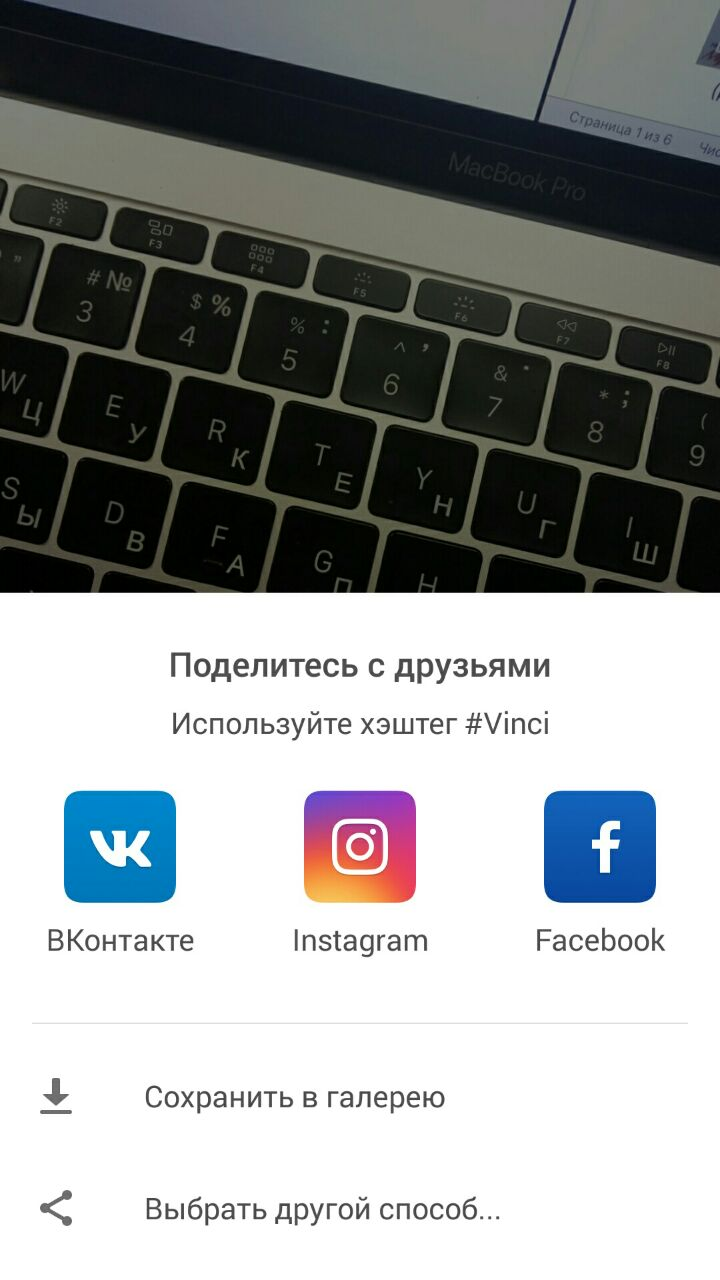
\includegraphics[width=0.3\linewidth]{pics/vinci3}
	\caption{Vinci}
	\label{fig:vinci}
\end{figure}

\subsubsection{Pixlr}

Особенностью интерфейса Pixlr (рисунок~\ref{fig:pixlr}),  в отличие от подобранных примеров, является присутствие стартового экрана, который, однако, несколько замедляет взаимодействие с приложением. Кнопки управление на экране камеры визуально неприятны и имеют непривычное соотношение размеров.

\begin{figure}[H]
	\centering
	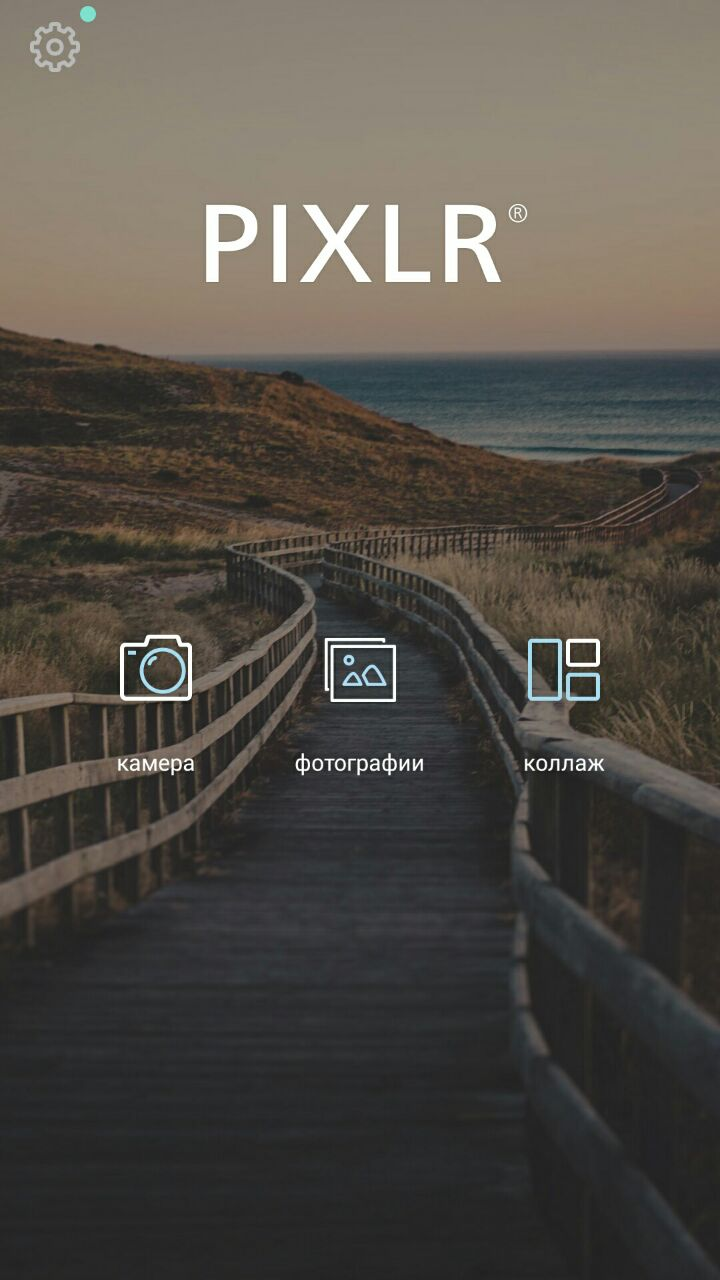
\includegraphics[width=0.45\linewidth]{pics/pixlr1}
	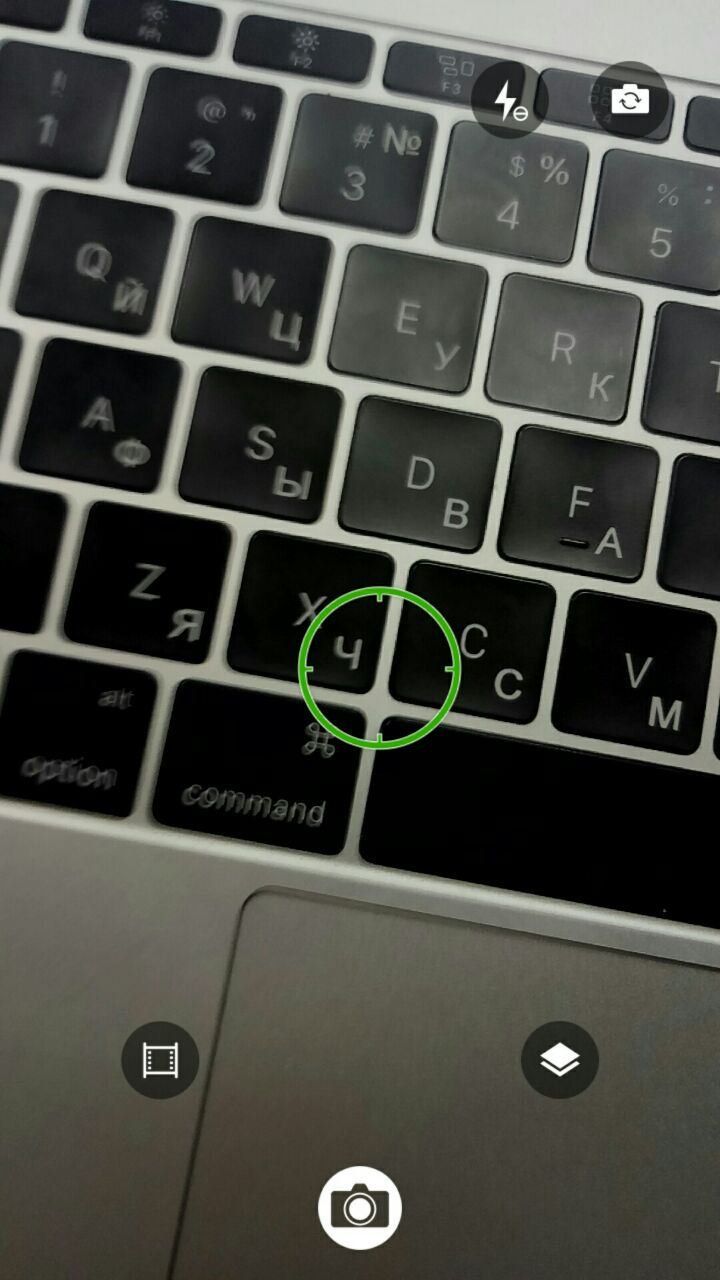
\includegraphics[width=0.45\linewidth]{pics/pixlr2}
	\caption{Pixlr}
	\label{fig:pixlr}
\end{figure}

\subsubsection{Snapster}

Как уже было сказано, Vinci и Snapster (рисунок~\ref{fig:snapster}) имеют примерно одинаковый уровень юзабилити, что объясняется одним и тем же авторством. В нижней части экрана размещен блок с последними снимками, но уже другим способ навигации - горизонтальной прокруткой (скроллом). Разработчик решил не внедрять кнопку настроек, нашлось место для полезно кнопки активации сетки. В целом, приложение Snapster, являясь экспериментальным проектом социальной сети VK, претерпело за время своего существования довольно сильные изменения. Если в первоначальном виде приложение дублировало основной функционал модуля «Фотографии» из социальной сети VK и расширяло его возможности, то сейчас, не сыскав популярности, было урезано до простенького фоторедактора.

\begin{figure}[H]
	\centering
	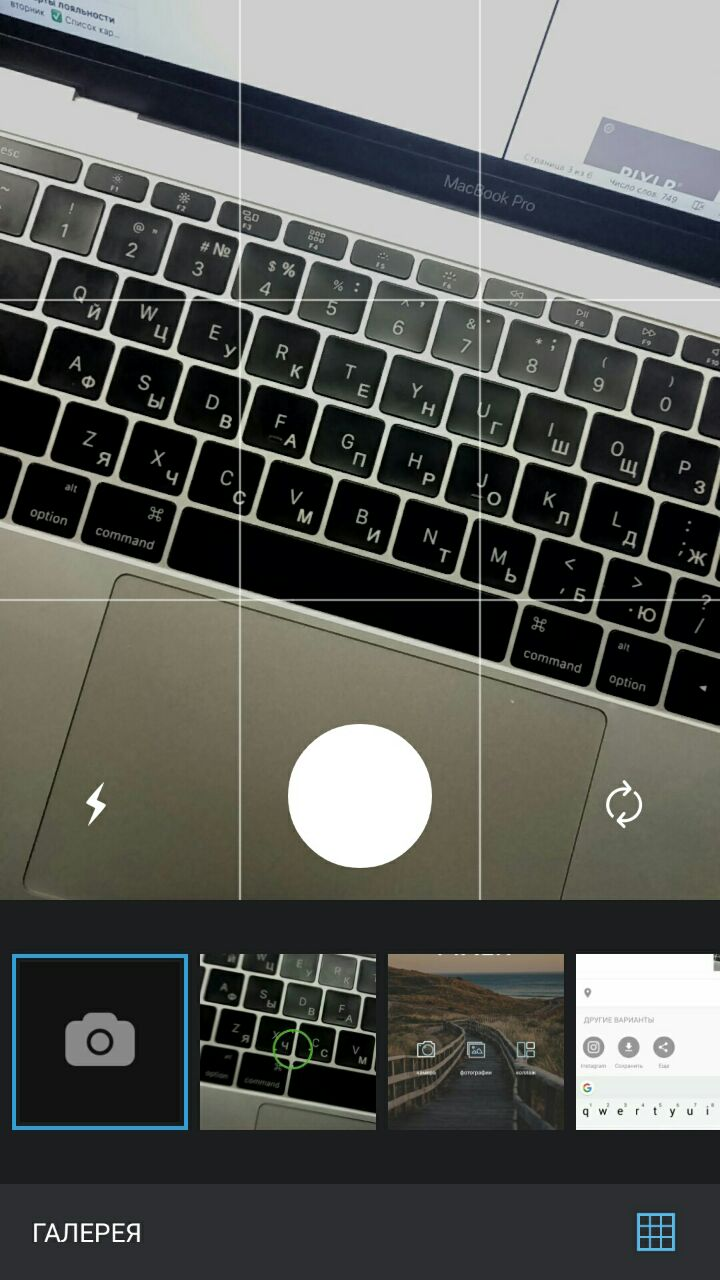
\includegraphics[width=0.45\linewidth]{pics/snapster1}
	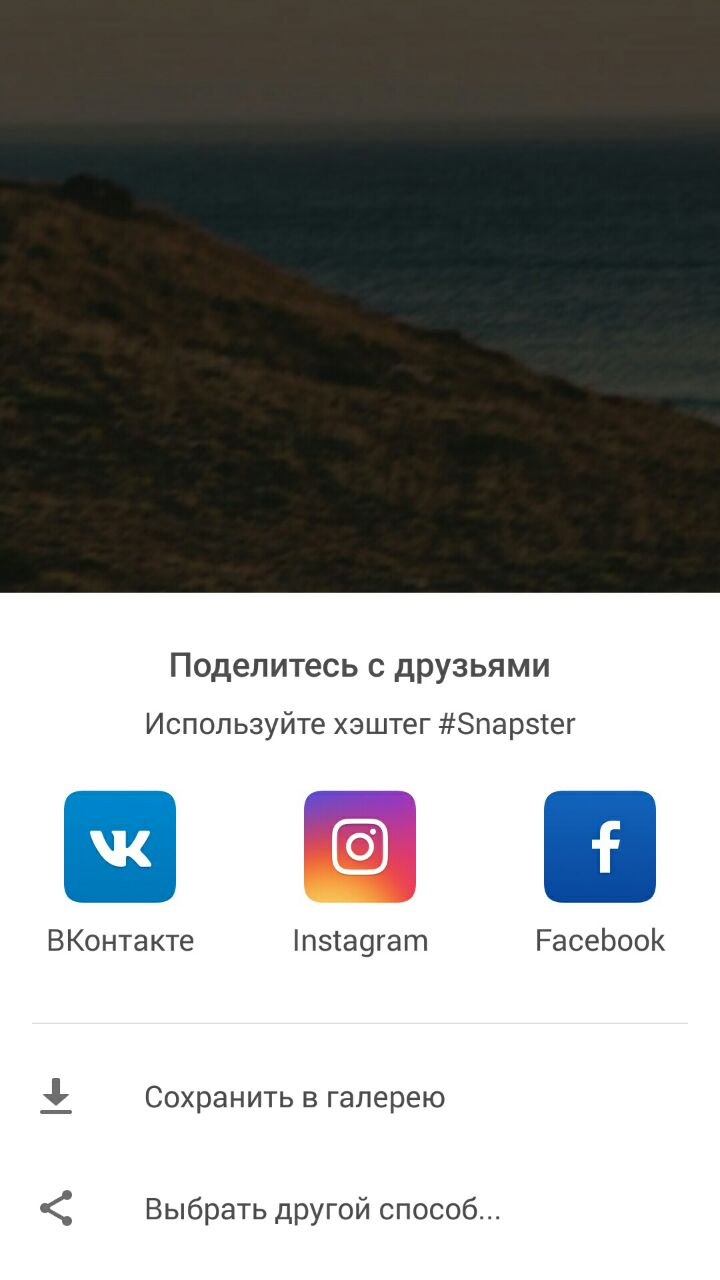
\includegraphics[width=0.45\linewidth]{pics/snapster2}
	\caption{Snapster}
	\label{fig:snapster}
\end{figure}

\subsection{Разработка пользовательского интерфейса мобильного приложения (UI/UX)}

Интерфейс Android-смартфона мобильного приложения для преобразования 2D фотографии в 3D вид выполнен в соответствии с гайдлайнами Material Design. Отступы, иконки и используемые шрифты полностью соответствуют руководству от Google~\cite{google}. 

Расположение элементов управление выполнено с учетом лучших особенностей приложений-аналогов.

На главный экран камеры (рисунок~\ref{fig:Artboard}) выведены следующие функции:

\begin{itemize}
	\item Спуск затвора;
	\item Выбор фото из галереи;
	\item Смена камеры;
	\item Управление вспышкой;
	\item Переход к настройкам и справке.
\end{itemize}

\begin{figure}[H]
	\centering
	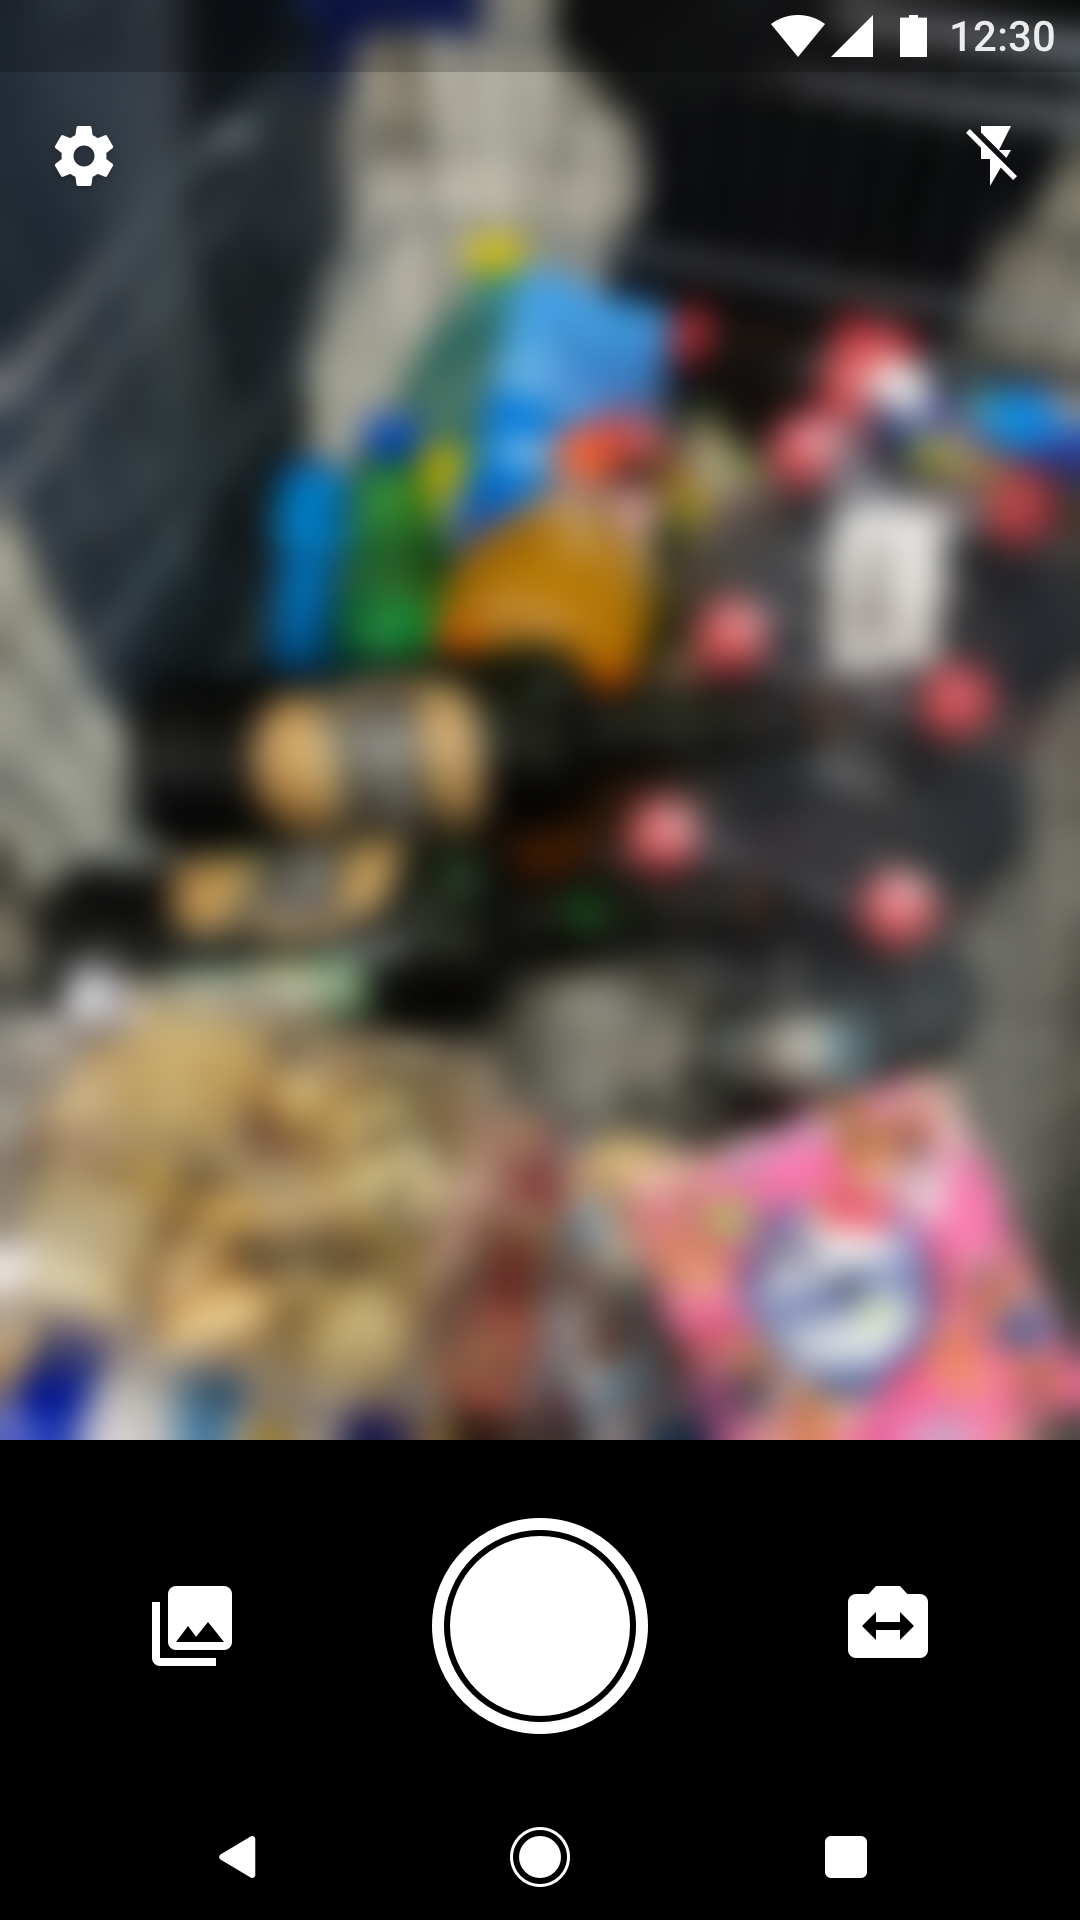
\includegraphics[width=0.6\linewidth]{pics/Artboard}
	\caption{Окно с камерой}
	\label{fig:Artboard}
\end{figure}

На экране с обработанной фотографией по нажатии кнопки «Далее» появляется bottom sheet (рисунок~\ref{fig:Artboard2}), включающий в себя быстрые функции шеринга и сохранения полученного фото в галерею.

\begin{figure}[H]
	\centering
	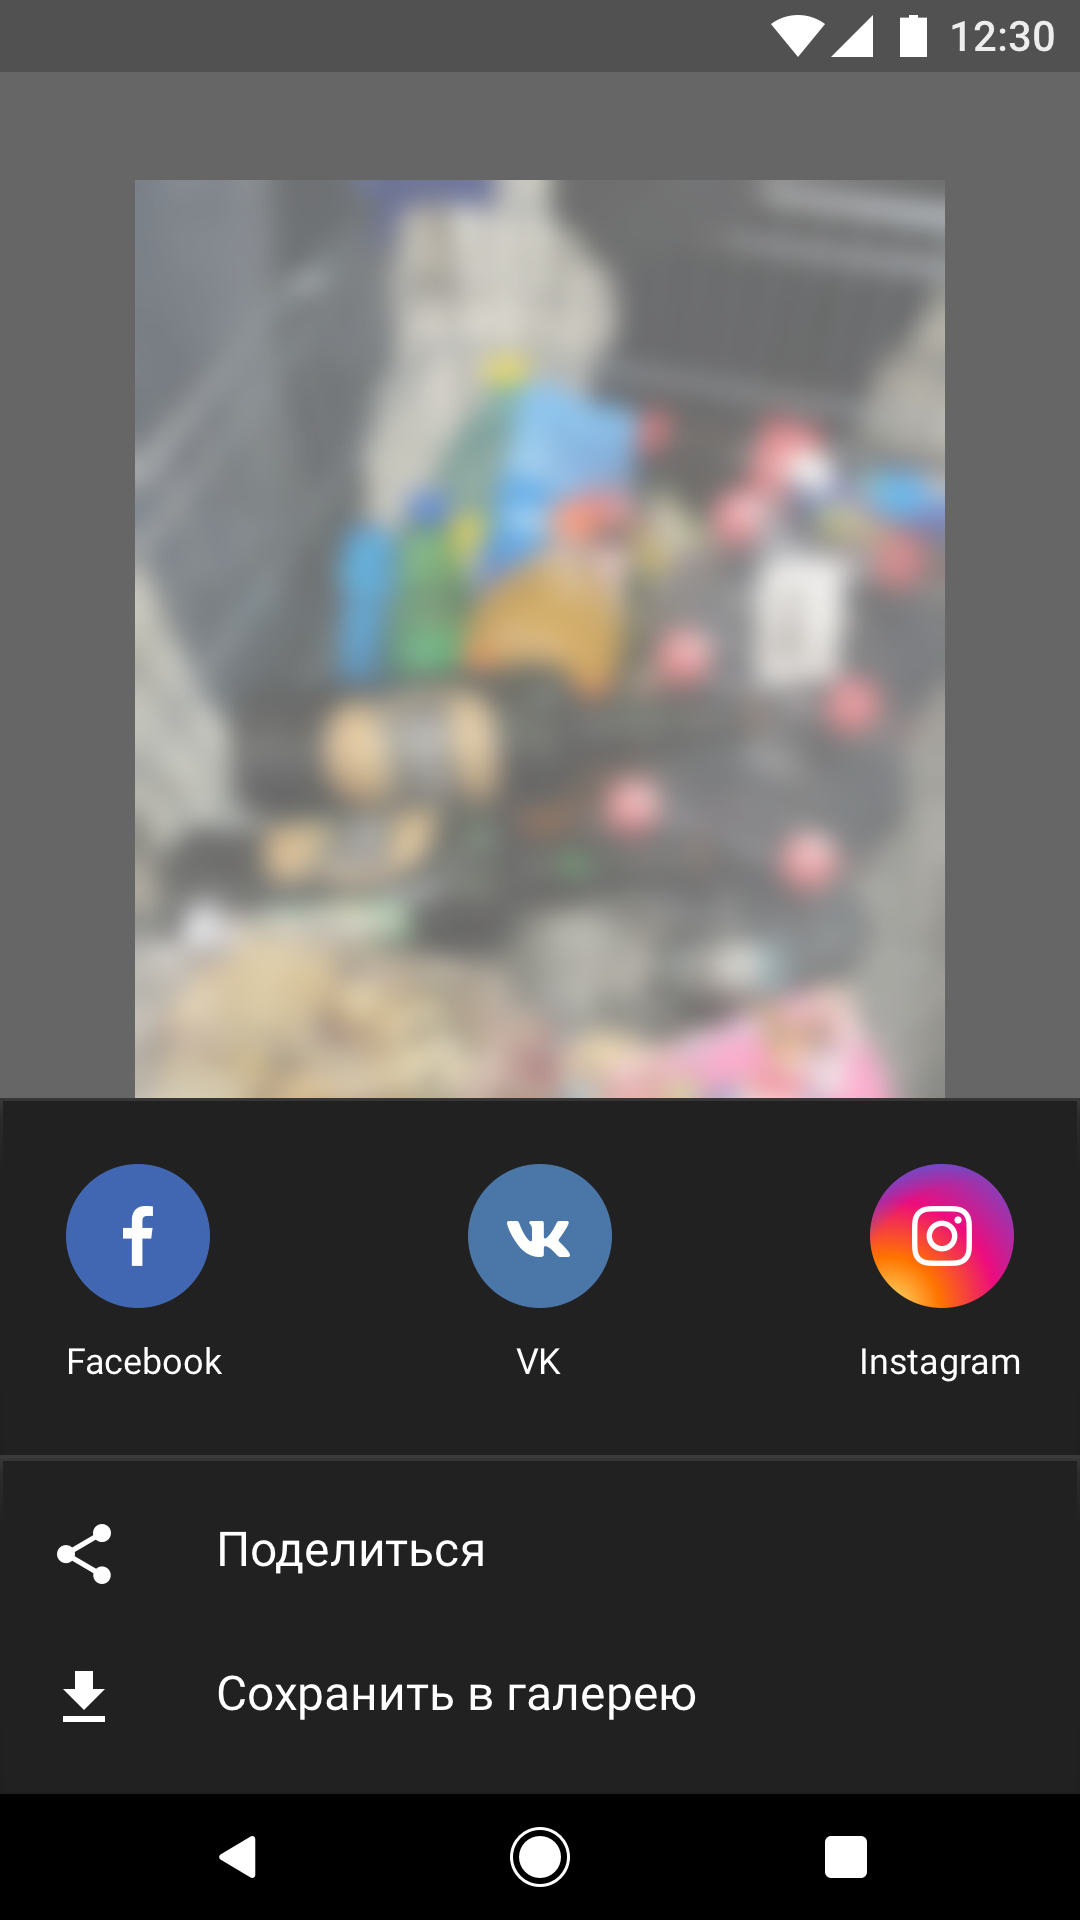
\includegraphics[width=0.6\linewidth]{pics/Artboard2}
	\caption{Окно с просмотром фото}
	\label{fig:Artboard2}
\end{figure}

При создании пользовательского интерфейса приложения были проанализированы современные, с аналогичным функционалом мобильные приложения в целом. Был сделан акцент на необходимости создания современного, функционального и не перегруженного пользовательского интерфейса. В результате проведенного анализа был создан пользовательский интерфейс мобильного приложения для преобразования 2D фотографий в 3D вид.